\documentclass{rpgcharsheet}
\begin{document}
%--------------------------------------------------------------------------------------------------------------------------------------------------------------------------------------------------------------------------
%%Classes
%\addclass														Class name, 	level,	 BAB,	 Fort,	 Ref, 	Will
\addclass	[calculate bab = true]										{ClassA}	{1}	{3/4}	{0}	{0}	{0}
\addclass	[calculate bab = true, calculate fort = true, calculate ref = true, calculate will = true]	{ClassB}	{10}	{1}	{1/2+2}	{1/3}	{1/2+2}
\addclass														{ClassC}	{1}	{1}	{1}	{2}	{0}

%\addcaster																				Class name	 Attribute
\addcaster	[offset = 0, first = 1, second = 1, third = 1, fourth = 1, fifth = 1, sixth = 1, seventh = 1, eighth = 1, ninth = 1]	{ClassC}	{int}

%\addspellmisc{Caster}{Spell level}{Type}{Value}
\addspellmisc{ClassC}{1}{untyped}{3}

%addpower[parent =, additional commands=]{Category (Domain, bloodline, etc)}{Caster}{Name}
\addpower{domain}{ClassC}{test}
\addpower{school}{ClassC}{testsd}
\addpower[parent = testsd]{school}{ClassC}{subtestsd}
\addpower{domain}{ClassC}{testdf}
\addpower[parent = test]{domain}{ClassC}{subtest1}
\addpower[parent = test]{domain}{ClassC}{subtest2}
\addpower{bloodline}{ClassC}{testb}
\addpower[parent = testb]{bloodline}{ClassC}{subtestb}
\addpower{something else}{ClassC}{testasd}
\addpower[parent = testasd]{something else}{ClassC}{aaaaaaaaa}

\favouredclass{ClassC}
%--------------------------------------------------------------------------------------------------------------------------------------------------------------------------------------------------------------------------
%%Player and character info 
\name{Name}
\playername{Player}
\alignment{Alignment}
\deity{Deity}
%Race name, race base speed
\race{Race}{30}
\homeland{Homeland}
%Fine, Diminutive, Tiny, Small, Medium, Large , Huge, Gargantuan, Colossal  (Capitalization is important)
\size{Large}
\gender{Gender}
\age{Age}
\height{Height}
\weight{Weight}
\hair{Hair}
\eyes{Eyes}

%--------------------------------------------------------------------------------------------------------------------------------------------------------------------------------------------------------------------------
%%HP without any modifiers
\setcounter{hpcount}{0}
\setcounter{favouredclasshpbonus}{0}

%--------------------------------------------------------------------------------------------------------------------------------------------------------------------------------------------------------------------------
%%Abilityscores
\setattribute{str}{18}
\setattribute{dex}{57}
\setattribute{con}{12}
\setattribute{int}{45}
\setattribute{wis}{10}
\setattribute{cha}{9}

\addtmpbonus{str}{2}

\addtypedbonus{str}{enhancement}{10}
\addtypedbonus{str}{enhancement}{3}

\addtypedbonus{spellresistance}{untyped}{3}

%--------------------------------------------------------------------------------------------------------------------------------------------------------------------------------------------------------------------------
%%Speed
%Swim, climb, fly
%\setspeed{Name (swim, climb, fly, burrow)}{Value}
\setspeed{swim}{0}
\setspeed{climb}{0}
\setspeed{fly}{0}
\setspeed{burrow}{0}

%--------------------------------------------------------------------------------------------------------------------------------------------------------------------------------------------------------------------------
%%Languages spoken
\addlanguages{Common}

%--------------------------------------------------------------------------------------------------------------------------------------------------------------------------------------------------------------------------
%%Skills
%		Name, 				trained only	 classskill	 Abillity mod  ranks	misc
\addskill	{acrobatics}				{0}		{1}		{dex}		{0}	{0}
\addskill	{appraise}				{0}		{0}		{int}		{0}	{0}
\addskill	{bluff}				{0}		{1}		{cha}		{0}	{0}
\addskill	{climb}				{0}		{1}		{str}		{0}	{0}
\addskill	{craft (armor)}			{0}		{1}		{int}		{0}	{0}
\addskill	{craft (bows)}			{0}		{1}		{int}		{0}	{0}
\addskill	{craft (weapons)}			{0}		{1}		{int}		{0}	{0}
\addskill	{diplomacy}				{0}		{1}		{cha}		{0}	{0}
\addskill	{disable device}			{1}		{0}		{dex}		{0}	{0}
\addskill	{disguise}				{0}		{0}		{cha}		{0}	{0}
\addskill	{escape artist}			{0}		{0}		{dex}		{0}	{0}
\addskill	{fly}					{0}		{0}		{dex}		{0}	{0}
\addskill	{handle animal}			{1}		{1}		{cha}		{0}	{0}
\addskill	{heal}					{0}		{0}		{wis}		{0}	{0}
\addskill	{intimidate}				{0}		{1}		{cha}		{0}	{0}
\addskill	{knowledge (arcana)}		{1}		{0}		{int}		{0}	{0}
\addskill	{knowledge (dungeoneering)}	{1}		{0}		{int}		{0}	{0}
\addskill	{knowledge (engineering)}	{1}		{0}		{int}		{0}	{0}
\addskill	{knowledge (geography)}		{1}		{0}		{int}		{0}	{0}
\addskill	{knowledge (history)}		{1}		{1}		{int}		{0}	{0}
\addskill	{knowledge (local)}			{1}		{0}		{int}		{0}	{0}
\addskill	{knowledge (nature)}		{1}		{0}		{int}		{10}	{0}
\addskill	{knowledge (nobility)}		{1}		{1}		{int}		{0}	{0}
\addskill	{knowledge (planes)}		{1}		{0}		{int}		{0}	{0}
\addskill	{knowledge (religion)}		{1}		{0}		{int}		{0}	{0}
\addskill	{linguistic}				{1}		{0}		{int}		{0}	{0}
\addskill	{perception}				{0}		{0}		{wis}		{0}	{0}
\addskill	{perform (string instruments)}	{0}		{1}		{cha}		{0}	{0}
\addskill	{profession (optional)}		{1}		{1}		{wis}		{0}	{0}
\addskill	{ride}					{0}		{1}		{dex}		{0}	{0}
\addskill	{sense motive}			{0}		{1}		{wis}		{0}	{0}
\addskill	{sleight of hand}			{1}		{0}		{dex}		{0}	{0}
\addskill	{spellcraft}				{1}		{0}		{int}		{0}	{0}
\addskill	{stealth}				{0}		{0}		{dex}		{0}	{0}
\addskill	{survival}				{0}		{1}		{wis}		{0}	{0}
\addskill	{swim}				{0}		{1}		{str}		{0}	{0}
\addskill	{use magic device}			{1}		{1}		{cha}		{10}	{0}

\addtypedbonus{stealth}{untyped}{\value{stealthsizemodcount}}
\addtypedbonus{fly}{untyped}{\value{flysizemodcount}}

%--------------------------------------------------------------------------------------------------------------------------------------------------------------------------------------------------------------------------

%% items/ Containers
%\addgear{Name}{Quantity/Volume}{Weight}
\addgear{Test}{10}{1}
\addgear[type = container]{Container}{10 lbs.}{1}

%Gear environment, adds gear to the item list.
%Content must be of the form: Name, Quantity, Weight; ...
\begin{Gear}
	ENV-Test, 10, 1;
\end{Gear}

%Container environment, adds container to the container list.
%The "weightless" parameter sets the weight of all items inside of the container to zero
%The "symbol" parameter adds a symbol to the container and its items
%Content must be of the form: Name, Volume/Quantity, Weight; ...
\begin{Container}[weightless = true, symbol = 1]{Bag of holding}{100}{12}
	ENV-Container-Test-1, 60, 2;
	ENV-Container-Test-2, 1, 2;
	ENV-Container-Test-3, 1, 2;
	ENV-Container-Test-4, 1, 2;
	ENV-Container-Test-5, 100, 2;
	ENV-Container-Test-6, 1, 2;
\end{Container}
\begin{Container}[symbol = 2]{Env-Container2}{500}{12}
	ENV-Container2-Test-1, 1, 2;
	ENV-Container2-Test-2, 1, 2;
	ENV-Container2-Test-3, 1, 2;
	ENV-Container2-Test-4, 1, 2;
	ENV-Container2-Test-5, 0, 2;
	ENV-Container2-Test-6, 1, 2;
\end{Container}
%--------------------------------------------------------------------------------------------------------------------------------------------------------------------------------------------------------------------------
%%AC-Items
%\addacitem{Name}{AC bonus}{Max dex}{Armor check penalty}{Spell failure}{Type (light, medium, heavy, shield, natural, misc)}{Weight}
\addacitem[enhancement = 5, notes = benevolent, base = Fullplate, category = heavy]{Test armor}{8}{5}{-6}{0}{heavy}{100}
\addacitem[category = shield]{Test shield}{1}{-}{-1}{35}{shield}{70}

%ACitem environment.
%Content must be of the form: [optional parameter] Name, AC bonus, Max dex, Armor check penalty, Spell failure, Type (light, medium, heavy, shield, natural, misc), Weight; ...
%Does not work
%\begin{ACitem}
%	Test natural, 5, -, 0, 0, natural, 70;
%\end{ACitem}

%--------------------------------------------------------------------------------------------------------------------------------------------------------------------------------------------------------------------------
%%Weapons
%\addweapon{Name}{Damage}{Critical}{Range}{Type}{Weight}{Ammo}
\addweapon[enhancement = 5, attack attribute = int, notes = note, base = Longsword, category = Heavy Blades]{Weapon int - str}{2d6}{18-20/x2}{-}{S}{12}{-}
\addweapon[masterwork = true, damage attribute = none]{Weapon str - none}{2d6}{18-20/x2}{-}{S}{12}{-}
\addweapon[attack attribute = dex, damage attribute = dex]{Weapon dex-dex}{2d6}{18-20/x2}{-}{S}{12}{-}


%Weapon environment
%Content must be of the form: [optional parameter] Name, Damage, Critical, Range, Type, Weight, Ammo; ...
\begin{Weapon}
	[attack attribute = int, notes = {flaming, hamster bane}, base = Longsword, category = Heavy Blades] Weapon int - str, 2d6, 18-20/x2, -, S, 12, -;
\end{Weapon}

%--------------------------------------------------------------------------------------------------------------------------------------------------------------------------------------------------------------------------
%%Worn magic items
%\addmagicitem{Name}{Type  (belt, body, chest, eyes, feet, hands, head, headband, neck, ring, shoulders, wrist)}{Additional commands}
\addmagicitem{Ring of protection}{ring}{\addacitem{Ring of protection}{1}{-}{0}{0}{deflection}{0}}
\addmagicitem{Masterwork tool (UMD)}{none}{\addtypedbonus{use magic device}{untyped}{2} \addgear{Masterwork tool (UMD)}{0}{1}}

%--------------------------------------------------------------------------------------------------------------------------------------------------------------------------------------------------------------------------
%Conditional Modifiers
%\addcondition[line break = true, comma = true]{Text}
\addcondition[line break = true, comma = true]{Locate traps: \writevalue{\value{ClassBlevelcount}/2}  perception}
\addcondition[line break = true, comma = true]{Locate traps: \writesignedvalue{\value{ClassBlevelcount}/2}  perception}
\addcondition[line break = true, comma = true]{Sample condition}

%Condition environment, adds conditions to the conditional modifier list.
%Content must be of the form: [optional parameter] Text; ...
\begin{Condition}
	[line break = true, comma = true] ENV-Sample condition;
\end{Condition}

%--------------------------------------------------------------------------------------------------------------------------------------------------------------------------------------------------------------------------
%%Feats
%\addfeat{Name}{Text}{additional commands}
\addfeat{Exotic Weapon Proficiency\linebreak Weapon}{You make attack rolls with the weapon normally.}{}
\addfeat{Skill Focus (Knowledge Nature)}{You get a +3 bonus on all checks involving the chosen skill. If you have 10 or more ranks in that skill, this bonus increases to +6.}{\ifthenelse{\value{knowledge (nature)skillrankcount}<10}{\addtypedbonus{knowledge (nature)}{untyped}{3}}{\addtypedbonus{knowledge (nature)}{untyped}{6}}}

%\unlockatlevel [companion, class], level, command
%Unlcok commands at a specific level
\unlockatlevel[class = ClassB]{5}{
	\addfeat{Cunning Initiative}{At 2nd level, an inquisitor adds her Wisdom modifier on initiative checks, in addition to her Dexterity modifier.}{\addtypedbonus{initiative}{untyped}{\maxof{\value{ClassBlevelcount}/2}{1}}}
}
\addfeat{Weapon focus Longsword}{You gain a +1 bonus on all attack rolls you make using the selected weapon.}{\addcategorybonus{Longsword}{attack}{1}}
\addfeat{Shield focus}{}{\addcategorybonus{shield}{ac bonus}{1}}

%--------------------------------------------------------------------------------------------------------------------------------------------------------------------------------------------------------------------------
%%Features
%\addfeature{Name}{Type (class, race, trait, flaw, etc)}{Text}{Uses}{additional commands}
\addfeature{Blatant}{flaws}{You suffer a -2 penalty to all Bluff, Disguise, and Stealth checks, as you find it difficult to conceal any aspect of your activities. Additionally, you cannot take 10 with these skills.}{-}{\addtypedbonus{bluff}{untyped}{-2}\addtypedbonus{disguise}{untyped}{-2}\addtypedbonus{stealth}{untyped}{-2}}

%\unlockatlevel [companion, class], level, command
%Unlcok commands at the specific level
\unlockatlevel[class = ClassA]{5}{
	\addfeature{ClassA Level 5}{ClassA}{}{-}{}
}
\unlockatlevel[class = ClassB]{10}{
	\addfeature{ClassB Level 10}{ClassB}{}{-}{}
}
\unlockatlevel[class = ClassC]{5}{
	\addfeature{ClassC Level 5}{ClassC}{}{-}{}
}

%------------------------------------------------------------------------------------------------------------------------does not work at this position
\addfeature{Armor training}{ClassC}{}{-}{\addcategorybonus{Fullplate}{penalty}{1}\addcategorybonus{heavy}{max dex}{1}}
\addfeature{Mind over metal}{}{use int instead of dex for armor class}{-}{\changeattribute{ac}{int}}

%--------------------------------------------------------------------------------------------------------------------------------------------------------------------------------------------------------------------------
%%Spells
%\addspell[Caster]{Level}{Name}{Text}{School}{Duration}{Range}{Save}{Target}
%Use close, medium, or long to calculate the range per caster level; Caster must be set

\addspell[caster = ClassC, caster level bonus = 0, prepared = true]{2}{Test1 +3 caster level}{Text}{School}{Instantaneous}{personal}{Reflex negates}{you}
\addspell[caster = ClassC, caster level bonus = 1]{6}{Test2 +1 caster level}{Text}{School}{Duration}{medium}{Reflex negates}{-}
\addspell[caster = ClassC, caster level bonus = 2, known = false]{2}{unknown Test3 +2 caster level}{Text}{School}{Duration}{long}{Reflex negates}{45 ft. cone}
\addspell{5}{Test1 +3 caster level}{Text}{School}{Duration}{close}{Reflex negates}{-}

%--------------------------------------------------------------------------------------------------------------------------------------------------------------------------------------------------------------------------
%%Notes
\addnote{Name}{Text}

%--------------------------------------------------------------------------------------------------------------------------------------------------------------------------------------------------------------------------
%%Currency
%\addcurrency	{Name}	{Carried}	{Weight}	{Stored}
\addcurrency	{Platinum}	{0}		{0.02}	{0}
\addcurrency	{Gold}		{650}		{0.02}	{0}
\addcurrency	{Silver}	{50}		{0.02}	{0}
\addcurrency	{Copper}	{9}		{0.02}	{0}

%--------------------------------------------------------------------------------------------------------------------------------------------------------------------------------------------------------------------------
%Companions
\addcompanion[load file = Companion]{Companion}%--------------------------------------------------------------------------------------------------------------------------------------------------------------------------------------------------------------------------
%Animate dead
\addtemplate{Undead}
{
	\addfeature[companion = \ID]{Darkvision 60ft.}{}{}{}{}
	%\addfeature[companion = \ID]{Immunity to all mind-affecting effects}{}{}{}{}
	%\addfeature[companion = \ID]{Immunity to bleed, death effects, disease, paralysis, poison, sleep effects, and stunning}{}{}{}{}
	%\addfeature[companion = \ID]{Immunity to any effect that requires a Fortitude save}{}{}{}{}
}

\addtemplate{Skeleton}
{
	\loadtemplate{Undead}
	\ifthenelse{\value{\ID sizeindex} = -1}{
		\addtypedbonus[companion = \ID]{ac}{natural}{1}
	}
	{
		\ifthenelse{\value{\ID sizeindex} = 0\OR \value{\ID sizeindex} = 1}{
			\addtypedbonus[companion = \ID]{ac}{natural}{2}
		}
		{
			\ifthenelse{\value{\ID sizeindex} = 2}{
				\addtypedbonus[companion = \ID]{ac}{natural}{3}
			}
			{
				\ifthenelse{\value{\ID sizeindex} = 3}{
					\addtypedbonus[companion = \ID]{ac}{natural}{6}
				}
				{
					\ifthenelse{\value{\ID sizeindex} > 3}{
						\addtypedbonus[companion = \ID]{ac}{natural}{10}
					}
					{
						\addtypedbonus[companion = \ID]{ac}{natural}{0}
					}
				}
			}
		}
	}
	\addtypedbonus[companion = \ID]{dex}{untyped}{2}
	\addfeat[companion = \ID]{Improved Initiative}{}{\addtypedbonus[companion = \ID]{initiative}{untyped}{4}}
	\global\expandafter\def\csname \ID damagereduction\endcsname{5/B}
}

\addtemplate{Bloody Skeleton}
{
	\loadtemplate{Skeleton}
	\setcounter{tmpcount7}{\value{\ID levelcount}/2}
	\addfeature[companion = \ID]{Fast Healing \arabic{tmpcount7}}{}{}{}{}
	\addfeature[companion = \ID]{Channel resistance +4}{}{}{}{}
	\addfeature[companion = \ID]{Deathless}{}{}{}{}
	\setattribute[companion = \ID]{cha}{14}
}

\addtemplate{Zombie}
{

}

\addtemplate{Incorporeal}
{
    \loadtemplate{Undead}
    \addtypedbonus[companion = \ID]{ac}{deflection}{\maxof{1}{\value{\ID chamodcount}}}
	\changeattribute[\ID]{cmb}{dex}
}

%%[optional parameter]{NAME}{HIT DICE}{HIT POINTS}{SIZE}{STR}{DEX}{TEMPLATE}{ADDITIONAL PARAMETERS}
\animatedead[number = 7, bucket = none]{Testecles}{12}{90}{Huge}{16}{10}{Bloody Skeleton}
{	
	\race[companion = \ID]{Storm giant}{30}
	\addtypedbonus[companion = \ID]{ac}{dodge}{1}
	\addtypedbonus[companion = \ID]{ac}{deflection}{2}
	\begin{Weapon}
		[companion = \ID, enhancement= 0, calculate size = 0, notes = trip] Katana (Large), 1d8, 18-20/x2, -, S, 12, -;
		[companion = \ID, enhancement= 0, calculate size = 0, notes = note] Katana (Large), 1d8, 18-20/x2, -, S, 12, -;
		[companion = \ID, enhancement= 0, calculate size = 0] Katana (Large), 1d8, 18-20/x2, -, S, 12, -;
	\end{Weapon}
}

\animatedead[number = 1, bucket = spell]{Greater Shadow}{9}{40}{Medium}{-}{20}{Incorporeal}
{	
	\race[companion = \ID]{Greater Shadow}{0}
	\setattribute[companion = \ID]{int}{6}
	\setattribute[companion = \ID]{wis}{12}
	\setattribute[companion = \ID]{cha}{15}
	\setspeed[companion = \ID]{fly}{40}
	\addfeat[companion = \ID]{Dodge}{}{\addtypedbonus[companion = \ID]{ac}{dodge}{1}}
	\addfeat[companion = \ID]{Flyby Attack}{}{}
	\addfeat[companion = \ID]{Mobility}{}{}
	\addfeat[companion = \ID]{Skill Focus (Perception, Stealth)}{}{}
	\addfeature[companion = \ID]{Strength Damage (Su)}{}{}{}{}
	\begin{Weapon}
		[companion = \ID, notes = {negative strength score $\Rightarrow$ DEATH, create spawn}, attack = \value{\ID babcount} + \value{\ID dexmodcount}] Katana (Large), 1d8 Strength, 20/x2, -, touch, 0, -;
	\end{Weapon}
}
\unitlength\textwidth
\divide\unitlength 420
\renewcommand\printsheet[1][]{
\ifthenelse{\equal{#1}{}}{}{
		\begin{picture}(420,0)
		\singletitlebox{-11.5}{10}{420}{10}{#1}	
		\end{picture}
	}

\noindent\begin{picture}(420,579)

\begin{picture}(0,0)
	\put(32,520){\hbox{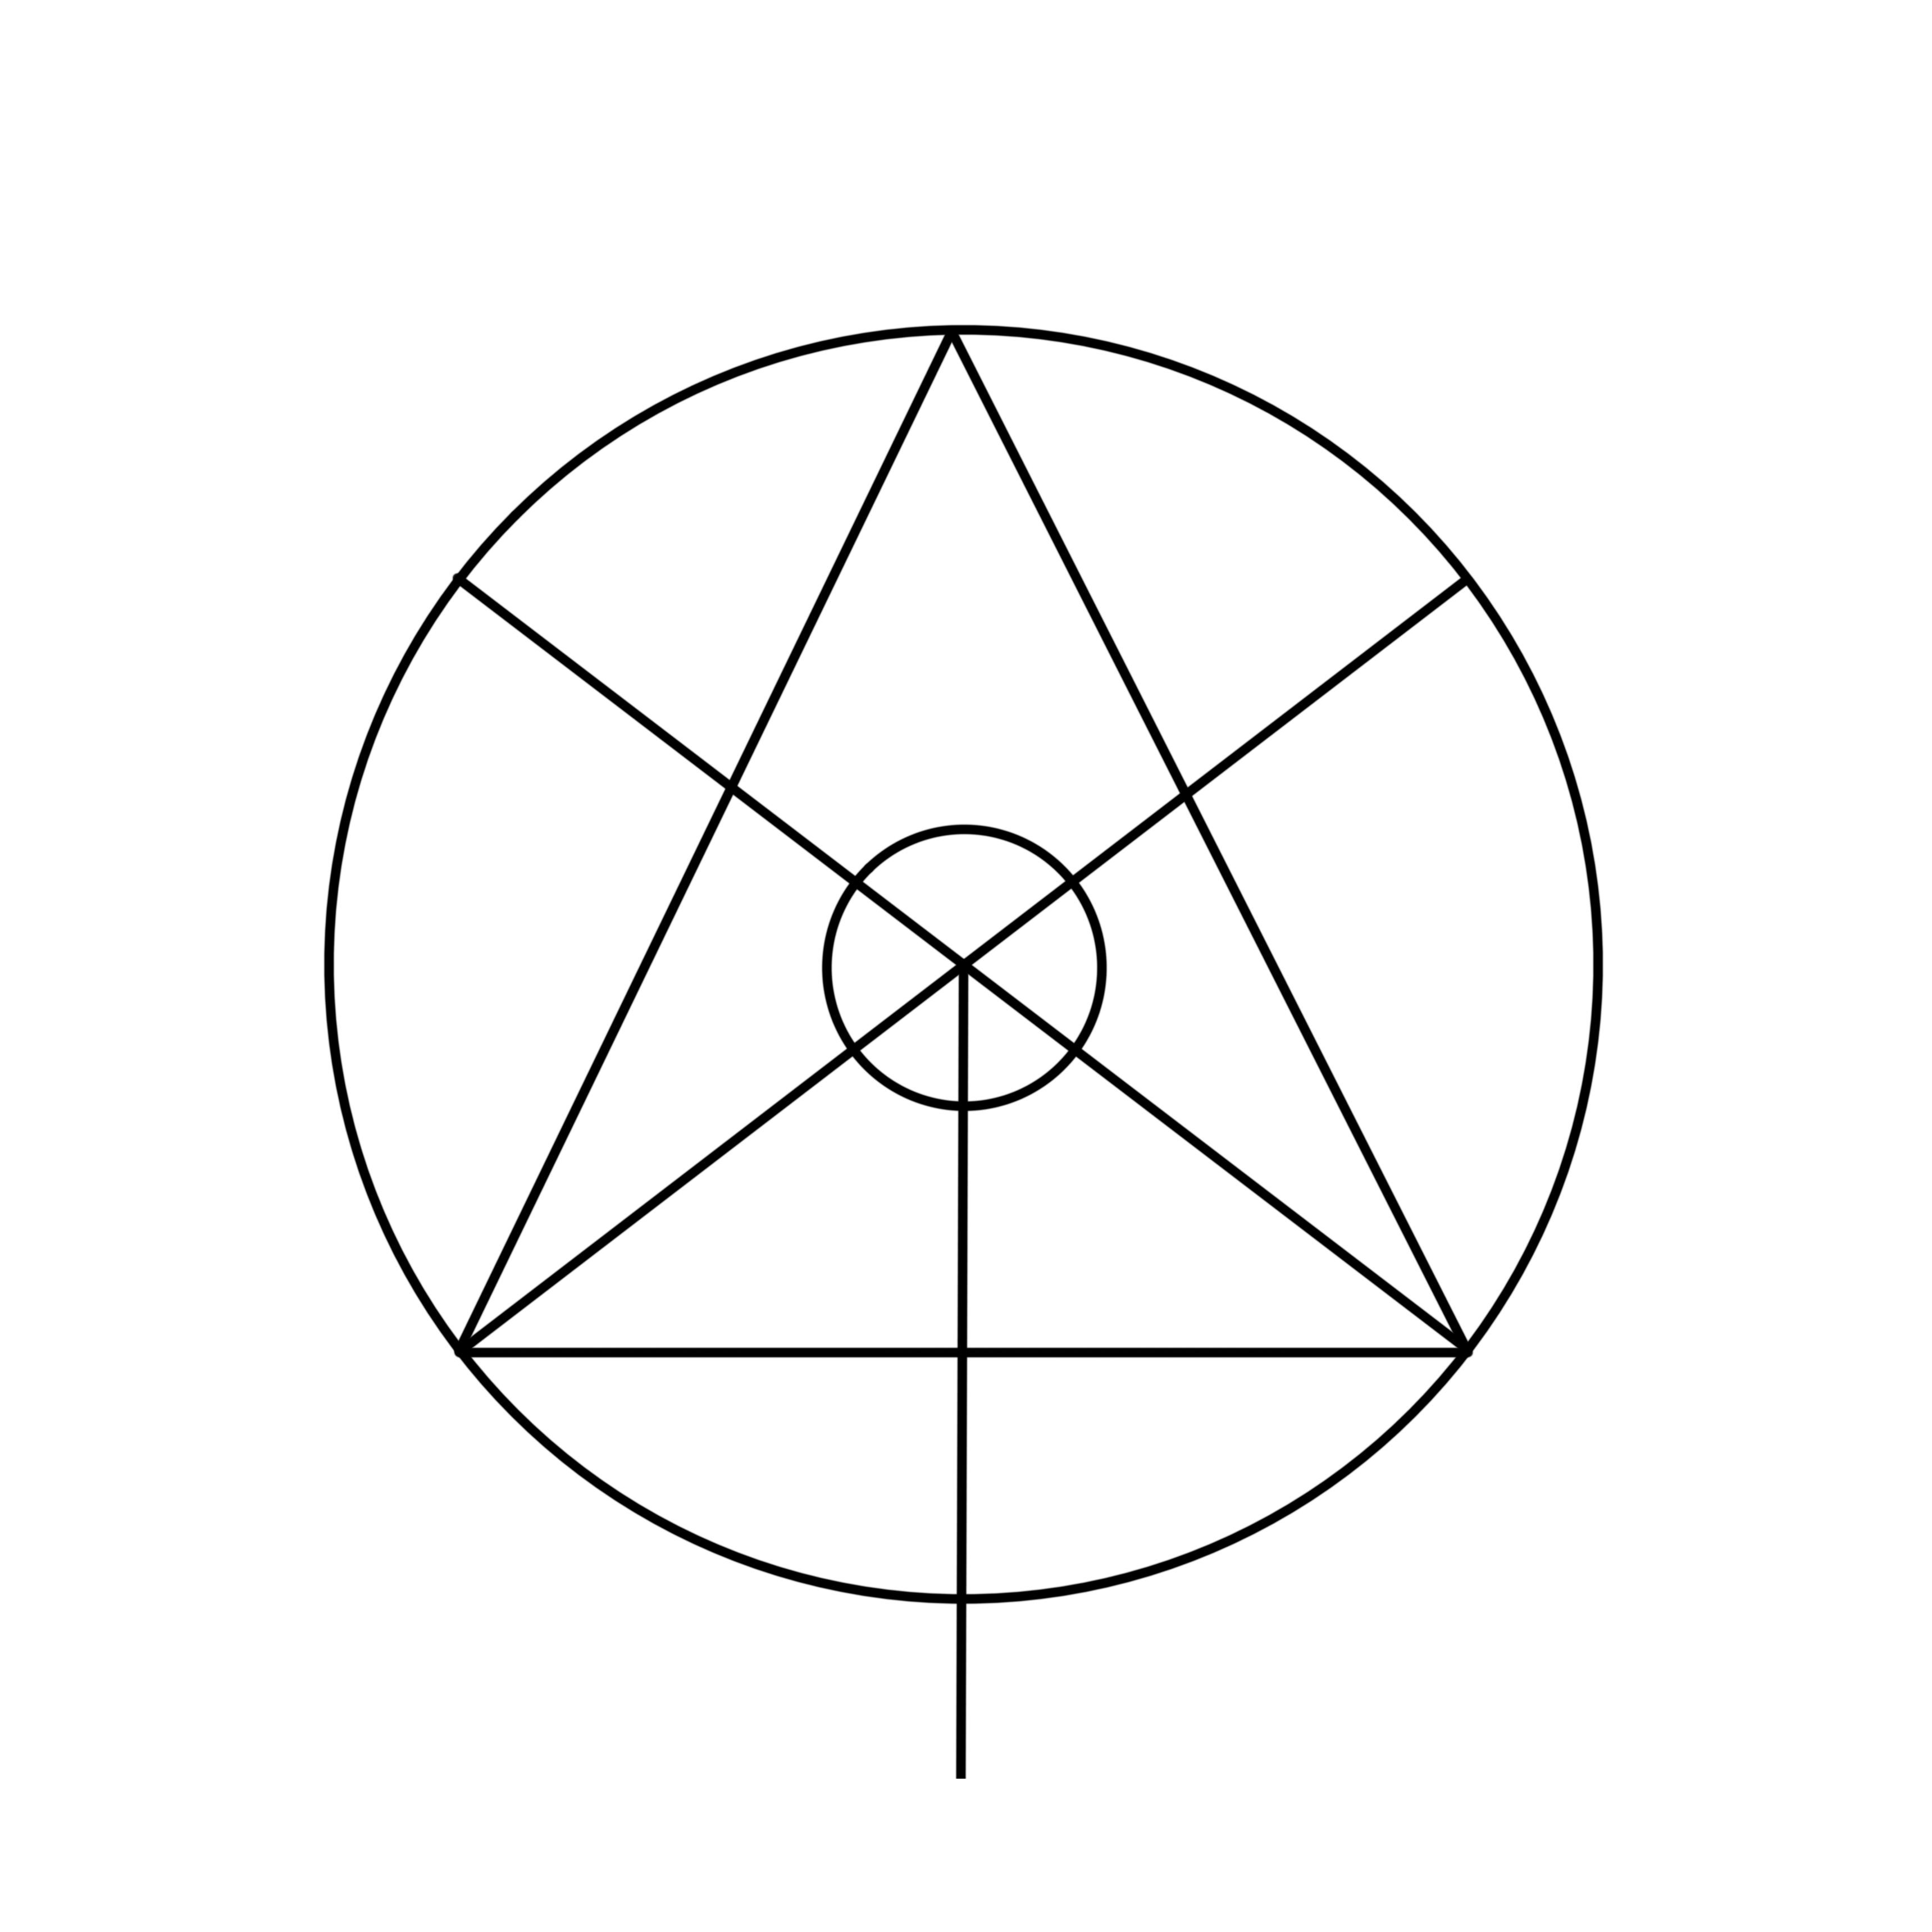
\includegraphics[scale=0.035]{Images/Logo}}}
\end{picture}


  \put(140,530){\renewcommand{\arraystretch}{1.5}
    \begin{tabular}[b]{D{46} D{23}  D{23}  D{23}  D{23}  D{23}  D{23}  D{23} }
      \multicolumn{3}{D{69}}{\csname #1charname\endcsname} &\multicolumn{3}{D{69}}{ \csname #1charalignment\endcsname} & \multicolumn{2}{D{46}}{\csname #1charplayername\endcsname} \\\cmidrule(rl){1-3}\cmidrule(rl){4-6}\cmidrule(rl){7-8}
      \multicolumn{4}{D{92}}{\csname #1classlist\endcsname} &\multicolumn{2}{D{46}}{\csname #1chardiety\endcsname} & \multicolumn{2}{D{46}}{\csname #1charhomeland\endcsname} \\\cmidrule(rl){1-4}\cmidrule(rl){5-6}\cmidrule(rl){7-8}
      \csname #1charrace\endcsname & \csname #1charsize\endcsname & \csname #1chargender\endcsname & \csname #1charage\endcsname & \csname #1charheight\endcsname & \csname #1charweight\endcsname & \csname #1charhair\endcsname & \csname #1chareyes\endcsname \\\cmidrule(rl){1-1}\cmidrule(rl){2-2}\cmidrule(rl){3-3}\cmidrule(rl){4-4}\cmidrule(rl){5-5}\cmidrule(rl){6-6}\cmidrule(rl){7-7}\cmidrule(rl){8-8}
    \end{tabular}}
  \put(140,529){\renewcommand{\arraystretch}{1.9}
    \begin{tabular}[b]{D{46} D{23}  D{23}  D{23}  D{23}  D{23}  D{23}  D{23} }
      \multicolumn{3}{D{69}}{\lfont character name} &  \multicolumn{3}{D{69}}{ \lfont alignment } & \multicolumn{2}{D{46}}{\lfont player name} \\
      \multicolumn{4}{D{92}}{\lfont character level} &\multicolumn{2}{D{46}}{\lfont deity} & \multicolumn{2}{D{46}}{\lfont homeland} \\
      \lfont race & \lfont size & \lfont gender & \lfont age & \lfont height & \lfont weight & \lfont hair & \lfont eyes \\
    \end{tabular}}

  \put(-0.8,438.5){%
    \setlength\fboxsep{0pt}\colorbox{black! 35}{%
      \makebox(68,80){
      }%
    }%
  }%

  %% Labels
  \put(0,512){\makebox(28,3){\tiny\scshape attribute}}
  \stretchlabels{33}{512}{102}{ability score,  ability modifier, Temp Adjustment, Temp Modifier}
  %% STR
  \titlebox{0}{500}{28}{STR}{strength}
\stretchattributes{33}{500}{102}{\arabic{#1strcount},\plusminus{#1strmodcount},\plusminus{#1strtmpcount},\plusminus{#1strtmpmodcount}}

  %% DEX
  \titlebox{0}{488}{28}{DEX}{dexterity}
  \stretchattributes{33}{488}{102}{\arabic{#1dexcount},\plusminus{#1dexmodcount},\plusminus{#1dextmpcount},\plusminus{#1dextmpmodcount}}
  
  %% CON
  \titlebox{0}{476}{28}{CON}{constitution}
  \stretchattributes{33}{476}{102}{\arabic{#1concount},\plusminus{#1conmodcount},\plusminus{#1contmpcount},\plusminus{#1contmpmodcount}}
  
  %% INT
  \titlebox{0}{464}{28}{INT}{intelligence}
  \stretchattributes{33}{464}{102}{\arabic{#1intcount},\plusminus{#1intmodcount},\plusminus{#1inttmpcount},\plusminus{#1inttmpmodcount}}

  %% WIS
  \titlebox{0}{452}{28}{WIS}{wisdom}
  \stretchattributes{33}{452}{102}{\arabic{#1wiscount},\plusminus{#1wismodcount},\plusminus{#1wistmpcount},\plusminus{#1wistmpmodcount}}

  %% CHA
  \titlebox{0}{440}{28}{CHA}{charisma}
  \stretchattributes{33}{440}{102}{\arabic{#1chacount},\plusminus{#1chamodcount},\plusminus{#1chatmpcount},\plusminus{#1chatmpmodcount}}

  %% HP
  \singletitlebox{107}{505}{26}{12}{HP}
  \put(137,505){\framebox(38,12){}}
  \put(137,512){\makebox(14,4){\tiny\scshape Total}}
  \put(137,505){\parbox[b][12\unitlength][c]{36\unitlength}{\raggedleft \chartotalhp}}
  \put(177,505){\framebox(28,12){}}
  \put(177,512){\makebox(8,4){\tiny\scshape DR}}

  %% little boxes
  \put(107,500){\makebox(36,4){\tiny\scshape wounds/current hp}}
  \put(107,480){\framebox(98,20){}}
  \put(109,480){\parbox[b][18\unitlength][t]{82\unitlength}{\tiny \textwoundscurrenthp}}
  \put(107,475){\makebox(36,4){\tiny\scshape nonleathal damage}}
  \put(107,455){\framebox(98,20){}}
  
  %% INIT
  \titlebox{107}{440}{43}{INITIATIVE}{modifier}
  \stretchequalattributes{152}{440}{206}{\arabic{\charinitmod},0}
  \stretchlabels{152}{434}{206}{TOTAL, dex modifier, misc modifier}
  
  %% AC
  \titlebox{0}{420}{27}{AC}{armour class}
  \equalattributes{25}{420}{10,\arabic{#1armorbonuscount},\arabic{#1shieldbonuscount},\arabic{#1dexbonuscount},\arabic{#1sizemodcount},\arabic{#1naturalbonuscount},\arabic{#1deflectionbonuscount},\arabic{#1miscbonuscount}}{20}
  \scaleattributelabels{25}{410}{TOTAL,default, armor bonus,shield bonus,dex \mbox{modifier},size \mbox{modifier},natural armour,\mbox{deflection} \mbox{modifier},misc \mbox{modifier}}{20}

  %% Touch, Flat footed
  \titlebox{0}{400}{35}{TOUCH}{armour class}
  \attributes{40}{400}{\calculatetouchac[#1]}
  \titlebox{60}{400}{55}{FLAT-FOOTED}{armour class}
  \attributes{120}{400}{\calculateflatfootedac[#1]} 
  \put(140,400){\framebox(65,9){}}
  \put(140,400){\parbox[b][8\unitlength][t]{65\unitlength}{\raggedleft \lfont modifiers}}

  %% fort, reflex and will
  \stretchlabels{60}{392}{205}{TOTAL, base save, ability modifier, magic modifier, misc modifier, temporary modifier}
  \titlebox{0}{380}{53}{fortitude}{(constitution)}
  \stretchequalattributes{60}{380}{205}{\arabic{#1fortcount},\arabic{#1conmodcount},0,\arabic{#1fortbonuscount},\arabic{#1forttmpcount}}
  \titlebox{0}{365}{53}{reflex}{(dexterity)}
  \stretchequalattributes{60}{365}{205}{\arabic{#1refcount},\arabic{#1dexmodcount},0,\arabic{#1refbonuscount},\arabic{#1reftmpcount}}
  \titlebox{0}{350}{53}{will}{(wisdom)}  
  \stretchequalattributes{60}{350}{205}{\arabic{#1willcount},\arabic{#1wismodcount},0,\arabic{#1willbonuscount},\arabic{#1willtmpcount}}

  %%Base attack bonus, spell resistance
  \singletitlebox{0}{329}{90}{11}{base attack bonus}
  \attributes{94}{330}{\arabic{#1babcount}}
  \singletitlebox{113}{329}{74}{11}{spell resistance}
  \attributes{190}{330}{0}
  
%%CMB and CMD
  \singletitlebox{0}{309}{21}{11}{cmb}
  \stretchequalattributes{25}{310}{130}{\arabic{#1babcount},\arabic{#1strmodcount},\arabic{#1specialsizemodcount}}
  \stretchlabels{25}{304}{130}{TOTAL, BAB,str mod., size mod.}
  \singletitlebox{0}{289}{21}{11}{cmd}
  \stretchequalattributes{25}{290}{130}{\arabic{#1babcount},\arabic{#1strmodcount},\arabic{#1dexmodcount},\arabic{#1specialsizemodcount} ,10}
  \stretchlabels{25}{284}{130}{TOTAL, BAB,str mod.,dex mod., size mod.,default}

  \singletitlebox{135}{284}{25}{35}{speed}
  % \put(135,284){\framebox(25,35){\uppercase{Speed}}}
  \put(165,310){\framebox(40,\boxheight){}}
  \put(164,311){\begin{tabular}[b]{F{17}E{2}F{16}E{2}}\arabic{#1base speedcount} &ft. & \basespeedsquares[#1]& sq.\end{tabular}}
  \put(165,307){\parbox[b][3\unitlength][b]{40\unitlength}{\centering\lfont base speed}}
  \put(165,297){\framebox(40,\boxheight){}}
  \put(164,298){\begin{tabular}[b]{F{17}E{2}F{16}E{2}}\armorspeed[#1] &ft. & \armorspeedsquares[#1]& sq.\end{tabular}}
  \put(165,294){\parbox[b][3\unitlength][b]{40\unitlength}{\centering\lfont with armour}}
  \put(165,284){\framebox(40,\boxheight){}}
  \put(164,285){\begin{tabular}[b]{F{17}E{2}@{\hspace{1ex}/\hspace{-1.6ex}}F{16}E{2}}\arabic{#1fly speedcount} &ft. & 0& \end{tabular}}
  \put(165,281){\parbox[b][3\unitlength][b]{40\unitlength}{\lfont\centering fly/manoeuvrability}}
  \put(135,271){\framebox(20,\boxheight){}}
  \put(134,272){\begin{tabular}[b]{F{16}E{2}}\arabic{#1swim speedcount} &ft.\end{tabular}}
  \put(135,267){\parbox[b][3\unitlength][b]{20\unitlength}{\centering\lfont swim}}
  \put(160,271){\framebox(20,\boxheight){}}
  \put(159,272){\begin{tabular}[b]{F{16}E{2}}\arabic{#1climb speedcount} &ft.\end{tabular}}
  \put(160,267){\parbox[b][3\unitlength][b]{20\unitlength}{\centering\lfont climb}}
  \put(185,271){\framebox(20,\boxheight){}}
  \put(184,272){\begin{tabular}[b]{F{16}E{2}}\arabic{#1burrow speedcount} &ft.\end{tabular}}
  \put(185,267){\parbox[b][3\unitlength][b]{20\unitlength}{\centering\lfont burrow}}
  \titlebox{0}{271}{50}{favoured}{Class}
  \put(55,271){\framebox(75,\boxheight){\footnotesize \charfavouredclass}}
 
\noindent\begin{picture}(0,0)
%%Weapons
 \put(-2,60){\begin{tabular}[t]{>{\centering}p{85\unitlength} >{\centering}p{55\unitlength} >{\centering}p{40\unitlength} >{\centering}p{40\unitlength} >{\centering}p{40\unitlength} >{\centering}p{20\unitlength} >{\centering}p{40\unitlength}>{\centering}p{25\unitlength} } 
\rowcolor{black}\leavevmode\color{white} \uppercase{Weapons} & \leavevmode\color{white}\lfont Attack modifiers & \leavevmode\color{white}\lfont damage & \leavevmode\color{white}\lfont critical &\leavevmode\color{white} \lfont range & \leavevmode\color{white}\lfont type &\leavevmode\color{white} \lfont weight &\leavevmode\color{white} \lfont ammo \tabularnewline\hline
\csname #1weaponlist\endcsname
\end{tabular}}

\end{picture}

  \put(215,508.89){
  \begin{tabular}[t]{A{2}A{10}B{80}A{21}B{7}A{21}A{7}A{21}A{7}A{21}}
    \rowcolor{black}& &\leavevmode\color{white}\footnotesize \scshape Skill Names&\leavevmode\color{white}\lfont Total\\ Bonus&&\leavevmode\color{white}\lfont Ability\\ Mod.&&\leavevmode\color{white}\lfont Ranks\\&&\leavevmode\color{white}\lfont Misc.\\ Mod.\ \tabularnewline
 \csname #1skilllist\endcsname 
&\lfont\mbox{\ooalign{$\checkmark$\cr\hidewidth$\square$\hidewidth\cr}}&\lfont Class Skill\hspace{2ex}  * trained only & & &\lfont Total & & \arabic{#1skillranks}
\end{tabular}}

  \singletitlebox{-2}{255}{205.4}{10}{Conditional Modifiers}
  \put(-1.7,170){\framebox(204.78,85){}}
  \put(0,210){\parbox[b][43\unitlength][t]{200\unitlength}{\itshape \csname #1conditionalmodlist\endcsname}}

  \singletitlebox{-2}{150}{205.4}{10}{Languages}
  \put(-1.7,85){\framebox(204.78,65){}}
  \put(0,110){\parbox[b][38\unitlength][t]{200\unitlength}{\itshape \tfont \csname #1languagelist\endcsname }}

\end{picture}

\newpagetitlebox[#1]

\noindent\begin{picture}(420,594)

  \singletitlebox{0}{594}{205}{10}{WORN MAGIC ITEM EQUIPMENT}
  \put(0,589){\begin{tabular}[t]{@{}p{30\unitlength} @{\hspace{1\unitlength}}>{\centering}p{169\unitlength}}
\\
  \hline
  \tfont Belt: & \csname #1magicitembelt\endcsname \tabularnewline
  \tfont Body: & \csname #1magicitembody\endcsname \tabularnewline
  \tfont Chest: & \csname #1magicitemchest\endcsname \tabularnewline
  \tfont Eyes: &  \csname #1magicitemeyes\endcsname \tabularnewline
  \tfont Feet: & \csname #1magicitemfeet\endcsname \tabularnewline
  \tfont Hands: & \csname #1magicitemhands\endcsname \tabularnewline
  \tfont Head: & \csname #1magicitemhead\endcsname \tabularnewline
  \tfont Headband: & \csname #1magicitemheadband\endcsname \tabularnewline
  \tfont Neck: & \csname #1magicitemneck\endcsname \tabularnewline
  \tfont Ring: & \csname #1magicitemringone\endcsname \tabularnewline
  \tfont Ring: & \csname #1magicitemringtwo\endcsname \tabularnewline
  \tfont Shoulders: & \csname #1magicitemshoulders\endcsname \tabularnewline
  \tfont Wrist: & \csname #1magicitemwrist\endcsname
 \end{tabular}}

 \singletitlebox{215}{594}{205}{10}{gear}
  \put(215,589){\begin{tabular}[t]{@{}p{150\unitlength} @{\hspace{1\unitlength}}>{\centering}p{29\unitlength}>{\centering}p{15\unitlength}@{}}\printgearitems[#1] \end{tabular}}

%%AC-items
  \put(0,449){\begin{tabular}[t]{>{\centering}p{40\unitlength} >{\centering}p{10\unitlength} >{\centering}p{10\unitlength} >{\centering}p{20\unitlength} >{\centering}p{20\unitlength} >{\centering}p{23\unitlength} >{\centering}p{17\unitlength} } \printacitems[#1] \end{tabular}}
  
  \put(0,325){\begin{tabular}[t]{>{\centering}p{40\unitlength} >{\centering}p{10\unitlength} >{\centering}p{10\unitlength} >{\centering}p{20\unitlength} >{\centering}p{20\unitlength} >{\centering}p{20\unitlength} >{\centering}p{17\unitlength} }\uppercase{totals} &\tfont \plusminus{#1acitemsbonus} &\tfont\ifthenelse{\value{#1maxdexbonuscount}<9999}{\plusminus{#1maxdexbonuscount}}{-} &\tfont \plusminus{#1acitemscheckpenalty} &\tfont \arabic{#1acitemsspellfailure}\% &&\tfont \arabic{#1acitemsweight}~lbs.  \end{tabular}}

\singletitlebox{0}{300}{205}{10}{Bags \& Containers}
  \put(0,295){\begin{tabular}[t]{@{}p{129\unitlength} @{\hspace{1\unitlength}}>{\centering}p{40\unitlength}>{\centering}p{25\unitlength}@{}}\printcontainers[#1] \end{tabular}}

\put(-2,210){
  \begin{tabular}[t]{>{\centering}p{42\unitlength}>{\centering}p{42\unitlength}>{\centering}p{42\unitlength}>{\centering}p{42\unitlength}}
\rowcolor{black} \leavevmode\color{white} \uppercase{Currency}& \leavevmode\lfont\color{white}Carried& \leavevmode\lfont\color{white}Carried weight&\leavevmode\lfont\color{white}Stored\tabularnewline
\csname #1currencylist\endcsname
\end{tabular}}

\singletitlebox{0}{140}{205}{10}{Carried Weight}
  \put(-2,135){ \begin{tabular}[t]{>{\centering}p{31\unitlength}>{\centering}p{31\unitlength}>{\centering}p{31\unitlength}>{\centering}p{31\unitlength}>{\centering}p{34\unitlength}}
  \lfont Armor \& Weapons &\lfont Currency & \lfont Equipment &\lfont Misc & \tfont\uppercase{Total} \tabularnewline\hline\\
  \printweight[#1]
\end{tabular}}

\singletitlebox{0}{90}{205}{10}{Loads \& Lift}
  \put(-2,85){ \begin{tabular}[t]{>{\centering}p{20\unitlength}>{\centering}p{20\unitlength}>{\centering}p{20\unitlength}>{\centering}p{20\unitlength}>{\centering}p{20\unitlength}>{\centering}p{20\unitlength}>{\centering}p{20\unitlength}}
  \lfont Light load&\lfont medium load & \lfont heavy load &\lfont & \lfont lift above head&\lfont lift of ground & \lfont drag \& push\tabularnewline\hline\\
 \printloadsandlift[#1]
\end{tabular}}

\singletitlebox{0}{30}{205}{10}{Experience Points}
  \put(-2,25){ \begin{tabular}[t]{|B{102}|B{102}|}
  \tfont\uppercase{ Current} &\tfont\uppercase{Next Level}\tabularnewline\hline
 & \\
 & \\
\hline
\end{tabular}}

\end{picture} 
\ifthenelse{\equal{\value{#1boolfeatures}}{0}}{}{
 \newpagetitlebox[#1]
\begin{longtable}{| p{.25\textwidth} | p{.666\textwidth} |p{.015\textwidth}| } 
\multicolumn{3}{c}{\singletitlebox{-210}{0}{420}{10}{features}}\endhead
\ifx\featurelist\emptylist
\else
\csname #1featurelist\endcsname
\fi
\end{longtable}
}

\ifthenelse{\equal{\value{#1boolfeats}}{0}}{}{
\newpagetitlebox[#1]
\begin{longtable}{| p{.25\textwidth} | p{.704\textwidth} |} 
\multicolumn{2}{c}{\singletitlebox{-210}{0}{420}{10}{feats}}\endhead
\hline
\csname #1featlist\endcsname
\end{longtable}
}
\csname #1printcasters\endcsname

\ifthenelse{\equal{\value{#1boolspells}}{0}}{}{
\newpagetitlebox[#1]
\begin{longtable}{| p{.015\textwidth}| p{.015\textwidth} | p{.483\textwidth+.038\textwidth}| p{.1\textwidth} | p{.07\textwidth} | p{.05\textwidth} | p{.03\textwidth}| p{.015\textwidth} |} 
\multicolumn{8}{c}{\singletitlebox{-210}{0}{420}{10}{spells}}\tabularnewline
\endhead 
\hline
\csname #1default0spelllist\endcsname
\csname #1default1spelllist\endcsname
\csname #1default2spelllist\endcsname
\csname #1default3spelllist\endcsname
\csname #1default4spelllist\endcsname
\csname #1default5spelllist\endcsname
\csname #1default6spelllist\endcsname
\csname #1default7spelllist\endcsname
\csname #1default8spelllist\endcsname
\csname #1default9spelllist\endcsname
\end{longtable}
}
}
\printsheet
\printcustomlists

\ifx \notelist\emptylist
	\else
	 \newpage
	\begin{longtable}{| p{.25\textwidth} | p{.704\textwidth} |} 
	\multicolumn{2}{c}{\singletitlebox{-210}{0}{420}{10}{notes}}\endhead
	\hline
	\notelist
	\end{longtable}
\fi

\printcompanions
\end{document}
%%% Local Variables: 
%%% mode: latex
%%% TeX-master: t
%%% End: 



